% Options for packages loaded elsewhere
\PassOptionsToPackage{unicode}{hyperref}
\PassOptionsToPackage{hyphens}{url}
%
\documentclass[
  11pt,
]{article}
\usepackage{amsmath,amssymb}
\usepackage{lmodern}
\usepackage{ifxetex,ifluatex}
\ifnum 0\ifxetex 1\fi\ifluatex 1\fi=0 % if pdftex
  \usepackage[T1]{fontenc}
  \usepackage[utf8]{inputenc}
  \usepackage{textcomp} % provide euro and other symbols
\else % if luatex or xetex
  \usepackage{unicode-math}
  \defaultfontfeatures{Scale=MatchLowercase}
  \defaultfontfeatures[\rmfamily]{Ligatures=TeX,Scale=1}
  \setmainfont[BoldFont = SF Pro Rounded Semibold, Scale =
MatchLowercase]{SF Pro Rounded}
  \setmathfont[]{SF Pro Rounded}
\fi
% Use upquote if available, for straight quotes in verbatim environments
\IfFileExists{upquote.sty}{\usepackage{upquote}}{}
\IfFileExists{microtype.sty}{% use microtype if available
  \usepackage[]{microtype}
  \UseMicrotypeSet[protrusion]{basicmath} % disable protrusion for tt fonts
}{}
\makeatletter
\@ifundefined{KOMAClassName}{% if non-KOMA class
  \IfFileExists{parskip.sty}{%
    \usepackage{parskip}
  }{% else
    \setlength{\parindent}{0pt}
    \setlength{\parskip}{6pt plus 2pt minus 1pt}}
}{% if KOMA class
  \KOMAoptions{parskip=half}}
\makeatother
\usepackage{xcolor}
\IfFileExists{xurl.sty}{\usepackage{xurl}}{} % add URL line breaks if available
\IfFileExists{bookmark.sty}{\usepackage{bookmark}}{\usepackage{hyperref}}
\hypersetup{
  pdftitle={Sample Exam},
  pdfauthor={Answers},
  hidelinks,
  pdfcreator={LaTeX via pandoc}}
\urlstyle{same} % disable monospaced font for URLs
\usepackage[margin=1.5in]{geometry}
\usepackage{longtable,booktabs,array}
\usepackage{calc} % for calculating minipage widths
% Correct order of tables after \paragraph or \subparagraph
\usepackage{etoolbox}
\makeatletter
\patchcmd\longtable{\par}{\if@noskipsec\mbox{}\fi\par}{}{}
\makeatother
% Allow footnotes in longtable head/foot
\IfFileExists{footnotehyper.sty}{\usepackage{footnotehyper}}{\usepackage{footnote}}
\makesavenoteenv{longtable}
\usepackage{graphicx}
\makeatletter
\def\maxwidth{\ifdim\Gin@nat@width>\linewidth\linewidth\else\Gin@nat@width\fi}
\def\maxheight{\ifdim\Gin@nat@height>\textheight\textheight\else\Gin@nat@height\fi}
\makeatother
% Scale images if necessary, so that they will not overflow the page
% margins by default, and it is still possible to overwrite the defaults
% using explicit options in \includegraphics[width, height, ...]{}
\setkeys{Gin}{width=\maxwidth,height=\maxheight,keepaspectratio}
% Set default figure placement to htbp
\makeatletter
\def\fps@figure{htbp}
\makeatother
\setlength{\emergencystretch}{3em} % prevent overfull lines
\providecommand{\tightlist}{%
  \setlength{\itemsep}{0pt}\setlength{\parskip}{0pt}}
\setcounter{secnumdepth}{-\maxdimen} % remove section numbering
\DeclareSymbolFont{symbolsC}{U}{txsyc}{m}{n}
\DeclareMathSymbol{\boxright}{\mathrel}{symbolsC}{128}
\usepackage{gensymb}
\usepackage{nicefrac}
\usepackage{caption}
\usepackage{istgame}
\usepackage{mathastext}
\ifluatex
  \usepackage{selnolig}  % disable illegal ligatures
\fi

\title{Sample Exam}
\author{Answers}
\date{}

\begin{document}
\maketitle

\hypertarget{truth-tables}{%
\subsection{Truth Tables}\label{truth-tables}}

For each of these sequents, do a truth table to test whether they are
valid. In each case, say whether they are valid.

\begin{enumerate}
\def\labelenumi{\arabic{enumi}.}
\tightlist
\item
  \(A \vee B, B \rightarrow A \vDash A\) - \textbf{VALID}
\end{enumerate}

\begin{tabular}{@{ }c@{ }@{ }c | c@{ }@{ }c@{ }@{ }c@{ }@{ }c@{ }@{ }c | c@{ }@{ }c@{ }@{ }c@{ }@{ }c@{ }@{ }c | c}
A & B &  & A & $\lor$ & B &  &  & B & $\rightarrow$ & A &  & A\\
\hline 
T & T &  & T & \textcolor{red}{T} & T &  &  & T & \textcolor{red}{T} & T &  & \textcolor{red}{T}\\
T & F &  & T & \textcolor{red}{T} & F &  &  & F & \textcolor{red}{T} & T &  & \textcolor{red}{T}\\
F & T &  & F & \textcolor{red}{T} & T &  &  & T & \textcolor{red}{F} & F &  & \textcolor{red}{F}\\
F & F &  & F & \textcolor{red}{F} & F &  &  & F & \textcolor{red}{T} & F &  & \textcolor{red}{F}\\
\end{tabular}

\begin{enumerate}
\def\labelenumi{\arabic{enumi}.}
\setcounter{enumi}{1}
\tightlist
\item
  \(\neg (A \wedge B), \neg (B \rightarrow A) \vDash A\) -
  \textbf{INVALID}
\end{enumerate}

\begin{tabular}{@{ }c@{ }@{ }c | c@{ }@{}c@{}@{ }c@{ }@{ }c@{ }@{ }c@{ }@{}c@{ } | c@{ }@{}c@{}@{ }c@{ }@{ }c@{ }@{ }c@{ }@{}c@{ } | c}
A & B & $\lnot$ & ( & A & $\land$ & B & ) & $\lnot$ & ( & B & $\rightarrow$ & A & ) & A\\
\hline 
T & T & \textcolor{red}{F} &  & T & T & T &  & \textcolor{red}{F} &  & T & T & T &  & \textcolor{red}{T}\\
T & F & \textcolor{red}{T} &  & T & F & F &  & \textcolor{red}{F} &  & F & T & T &  & \textcolor{red}{T}\\
F & T & \textcolor{red}{T} &  & F & F & T &  & \textcolor{red}{T} &  & T & F & F &  & \textcolor{red}{F}\\
F & F & \textcolor{red}{T} &  & F & F & F &  & \textcolor{red}{F} &  & F & T & F &  & \textcolor{red}{F}\\
\end{tabular}

\begin{enumerate}
\def\labelenumi{\arabic{enumi}.}
\setcounter{enumi}{2}
\tightlist
\item
  \(A \rightarrow B \vDash B \rightarrow A\) - \textbf{INVALID}
\end{enumerate}

\begin{tabular}{@{ }c@{ }@{ }c | c@{ }@{ }c@{ }@{ }c@{ }@{ }c@{ }@{ }c | c@{ }@{ }c@{ }@{ }c@{ }@{ }c@{ }@{ }c}
A & B &  & A & $\rightarrow$ & B &  &  & B & $\rightarrow$ & A & \\
\hline 
T & T &  & T & \textcolor{red}{T} & T &  &  & T & \textcolor{red}{T} & T & \\
T & F &  & T & \textcolor{red}{F} & F &  &  & F & \textcolor{red}{T} & T & \\
F & T &  & F & \textcolor{red}{T} & T &  &  & T & \textcolor{red}{F} & F & \\
F & F &  & F & \textcolor{red}{T} & F &  &  & F & \textcolor{red}{T} & F & \\
\end{tabular}

\newpage

\begin{enumerate}
\def\labelenumi{\arabic{enumi}.}
\setcounter{enumi}{3}
\tightlist
\item
  \(A \rightarrow (B \vee C), C \rightarrow (A \vee B) \vDash B\) -
  \textbf{INVALID}
\end{enumerate}

\begin{tabular}{@{ }c@{ }@{ }c@{ }@{ }c | c@{ }@{ }c@{ }@{ }c@{ }@{}c@{}@{ }c@{ }@{ }c@{ }@{ }c@{ }@{}c@{}@{ }c | c@{ }@{ }c@{ }@{ }c@{ }@{}c@{}@{ }c@{ }@{ }c@{ }@{ }c@{ }@{}c@{}@{ }c | c}
A & B & C &  & A & $\rightarrow$ & ( & B & $\lor$ & C & ) &  &  & C & $\rightarrow$ & ( & A & $\lor$ & B & ) &  & B\\
\hline 
T & T & T &  & T & \textcolor{red}{T} &  & T & T & T &  &  &  & T & \textcolor{red}{T} &  & T & T & T &  &  & \textcolor{red}{T}\\
T & T & F &  & T & \textcolor{red}{T} &  & T & T & F &  &  &  & F & \textcolor{red}{T} &  & T & T & T &  &  & \textcolor{red}{T}\\
T & F & T &  & T & \textcolor{red}{T} &  & F & T & T &  &  &  & T & \textcolor{red}{T} &  & T & T & F &  &  & \textcolor{red}{F}\\
T & F & F &  & T & \textcolor{red}{F} &  & F & F & F &  &  &  & F & \textcolor{red}{T} &  & T & T & F &  &  & \textcolor{red}{F}\\
F & T & T &  & F & \textcolor{red}{T} &  & T & T & T &  &  &  & T & \textcolor{red}{T} &  & F & T & T &  &  & \textcolor{red}{T}\\
F & T & F &  & F & \textcolor{red}{T} &  & T & T & F &  &  &  & F & \textcolor{red}{T} &  & F & T & T &  &  & \textcolor{red}{T}\\
F & F & T &  & F & \textcolor{red}{T} &  & F & T & T &  &  &  & T & \textcolor{red}{F} &  & F & F & F &  &  & \textcolor{red}{F}\\
F & F & F &  & F & \textcolor{red}{T} &  & F & F & F &  &  &  & F & \textcolor{red}{T} &  & F & F & F &  &  & \textcolor{red}{F}\\
\end{tabular}

\hypertarget{truth-trees}{%
\subsection{Truth Trees}\label{truth-trees}}

For each of these sequents, do a truth table to test whether they are
valid. In each case, say whether they are valid.

\begin{enumerate}
\def\labelenumi{\arabic{enumi}.}
\setcounter{enumi}{4}
\tightlist
\item
  \(A \vee B, B \rightarrow A \vDash A\)
\end{enumerate}

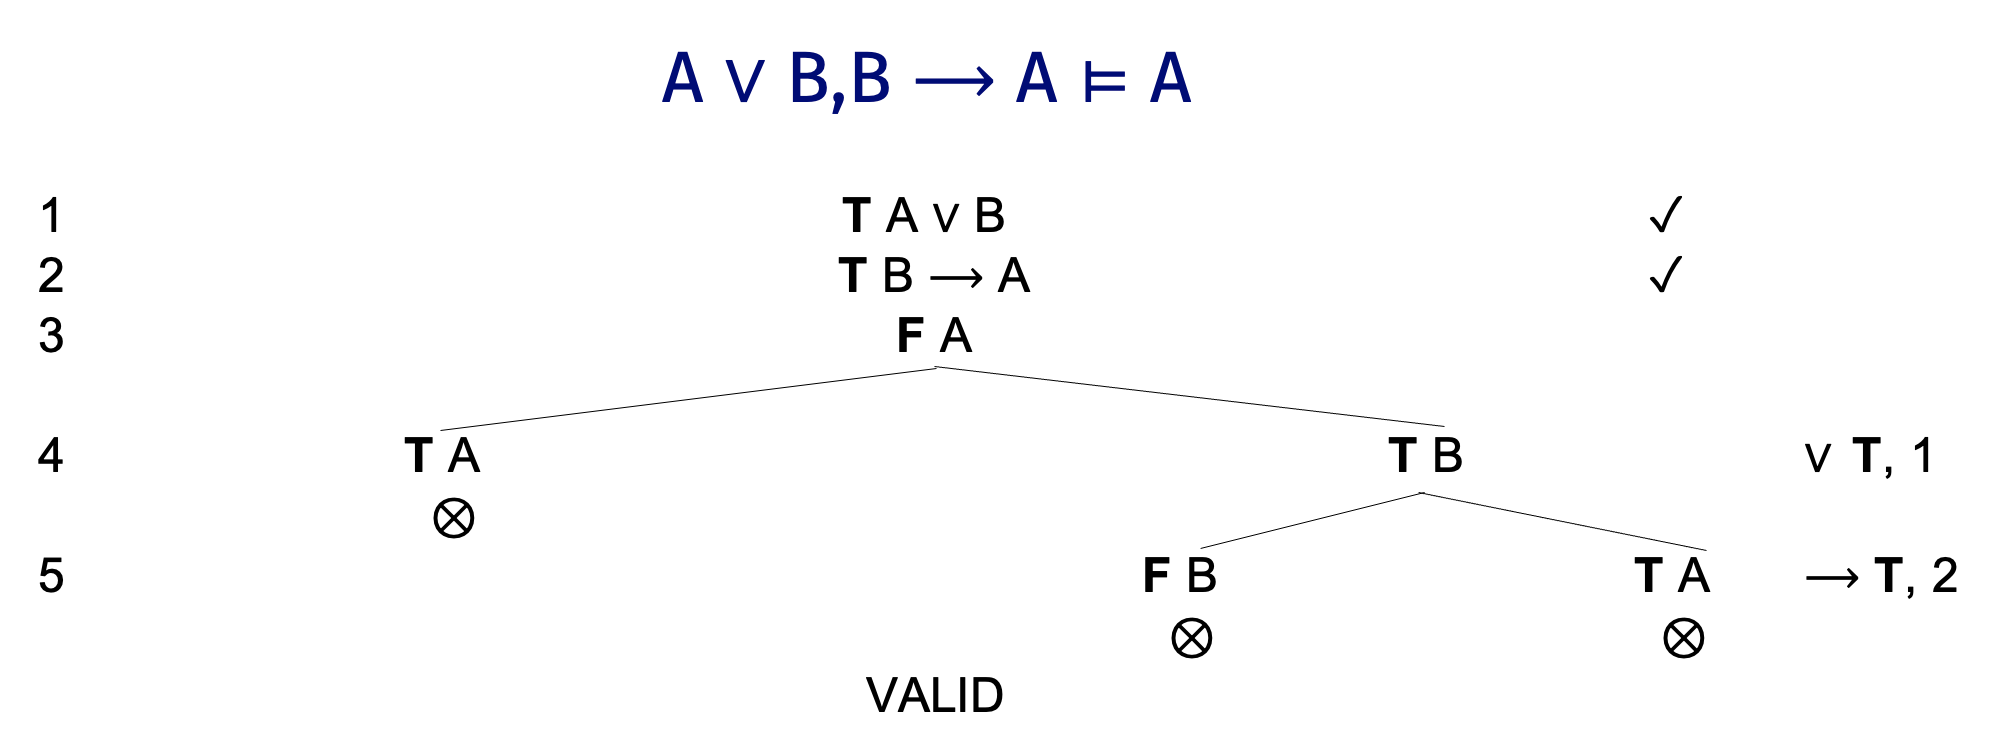
\includegraphics{q05.png}

\begin{enumerate}
\def\labelenumi{\arabic{enumi}.}
\setcounter{enumi}{5}
\tightlist
\item
  \(\neg (A \wedge B), \neg (B \rightarrow A) \vDash A\)
\end{enumerate}

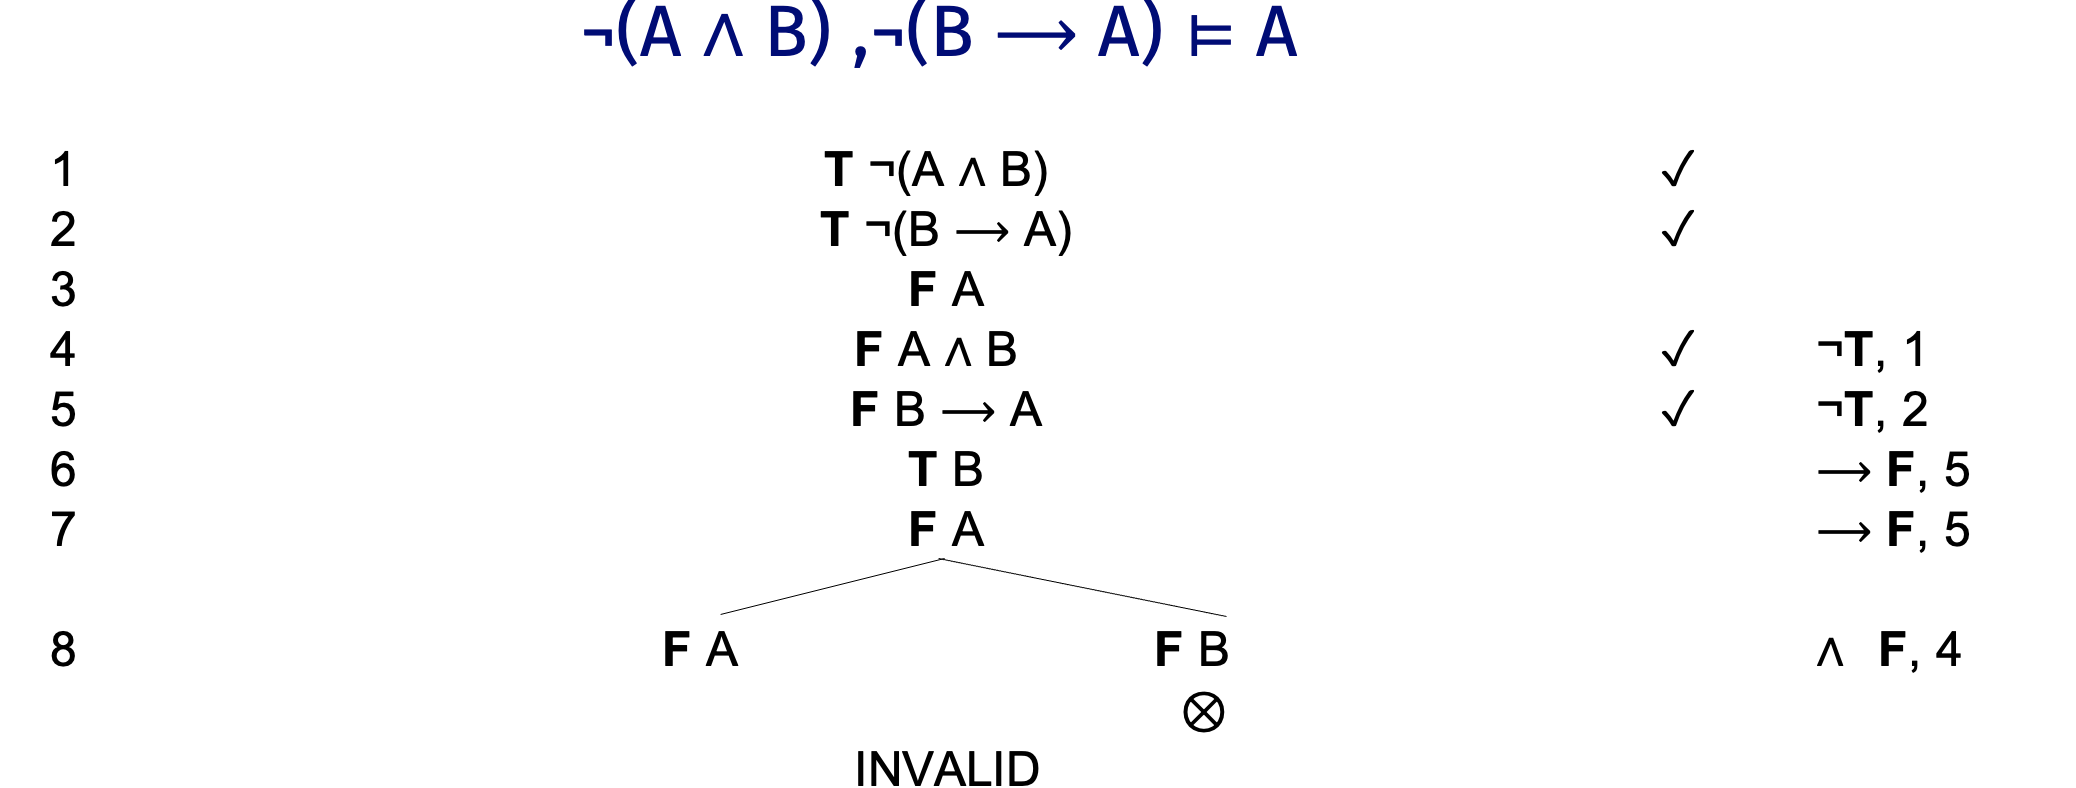
\includegraphics{q06.png}

\begin{enumerate}
\def\labelenumi{\arabic{enumi}.}
\setcounter{enumi}{6}
\tightlist
\item
  \(A \rightarrow B \vDash B \rightarrow A\)
\end{enumerate}

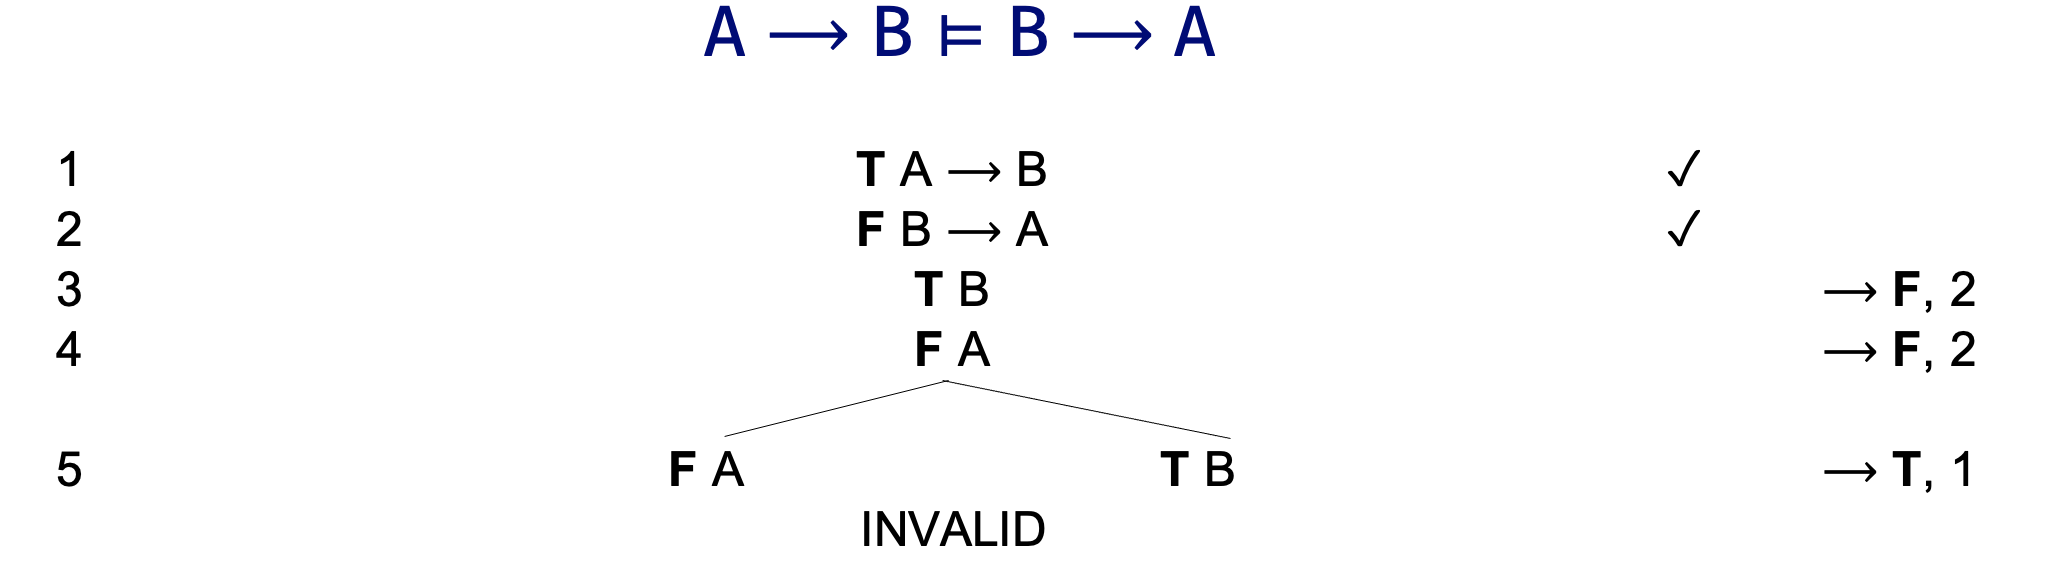
\includegraphics{q07.png}

\begin{enumerate}
\def\labelenumi{\arabic{enumi}.}
\setcounter{enumi}{7}
\tightlist
\item
  \(A \rightarrow (B \vee C), C \rightarrow (A \vee B) \vDash B\)
\end{enumerate}

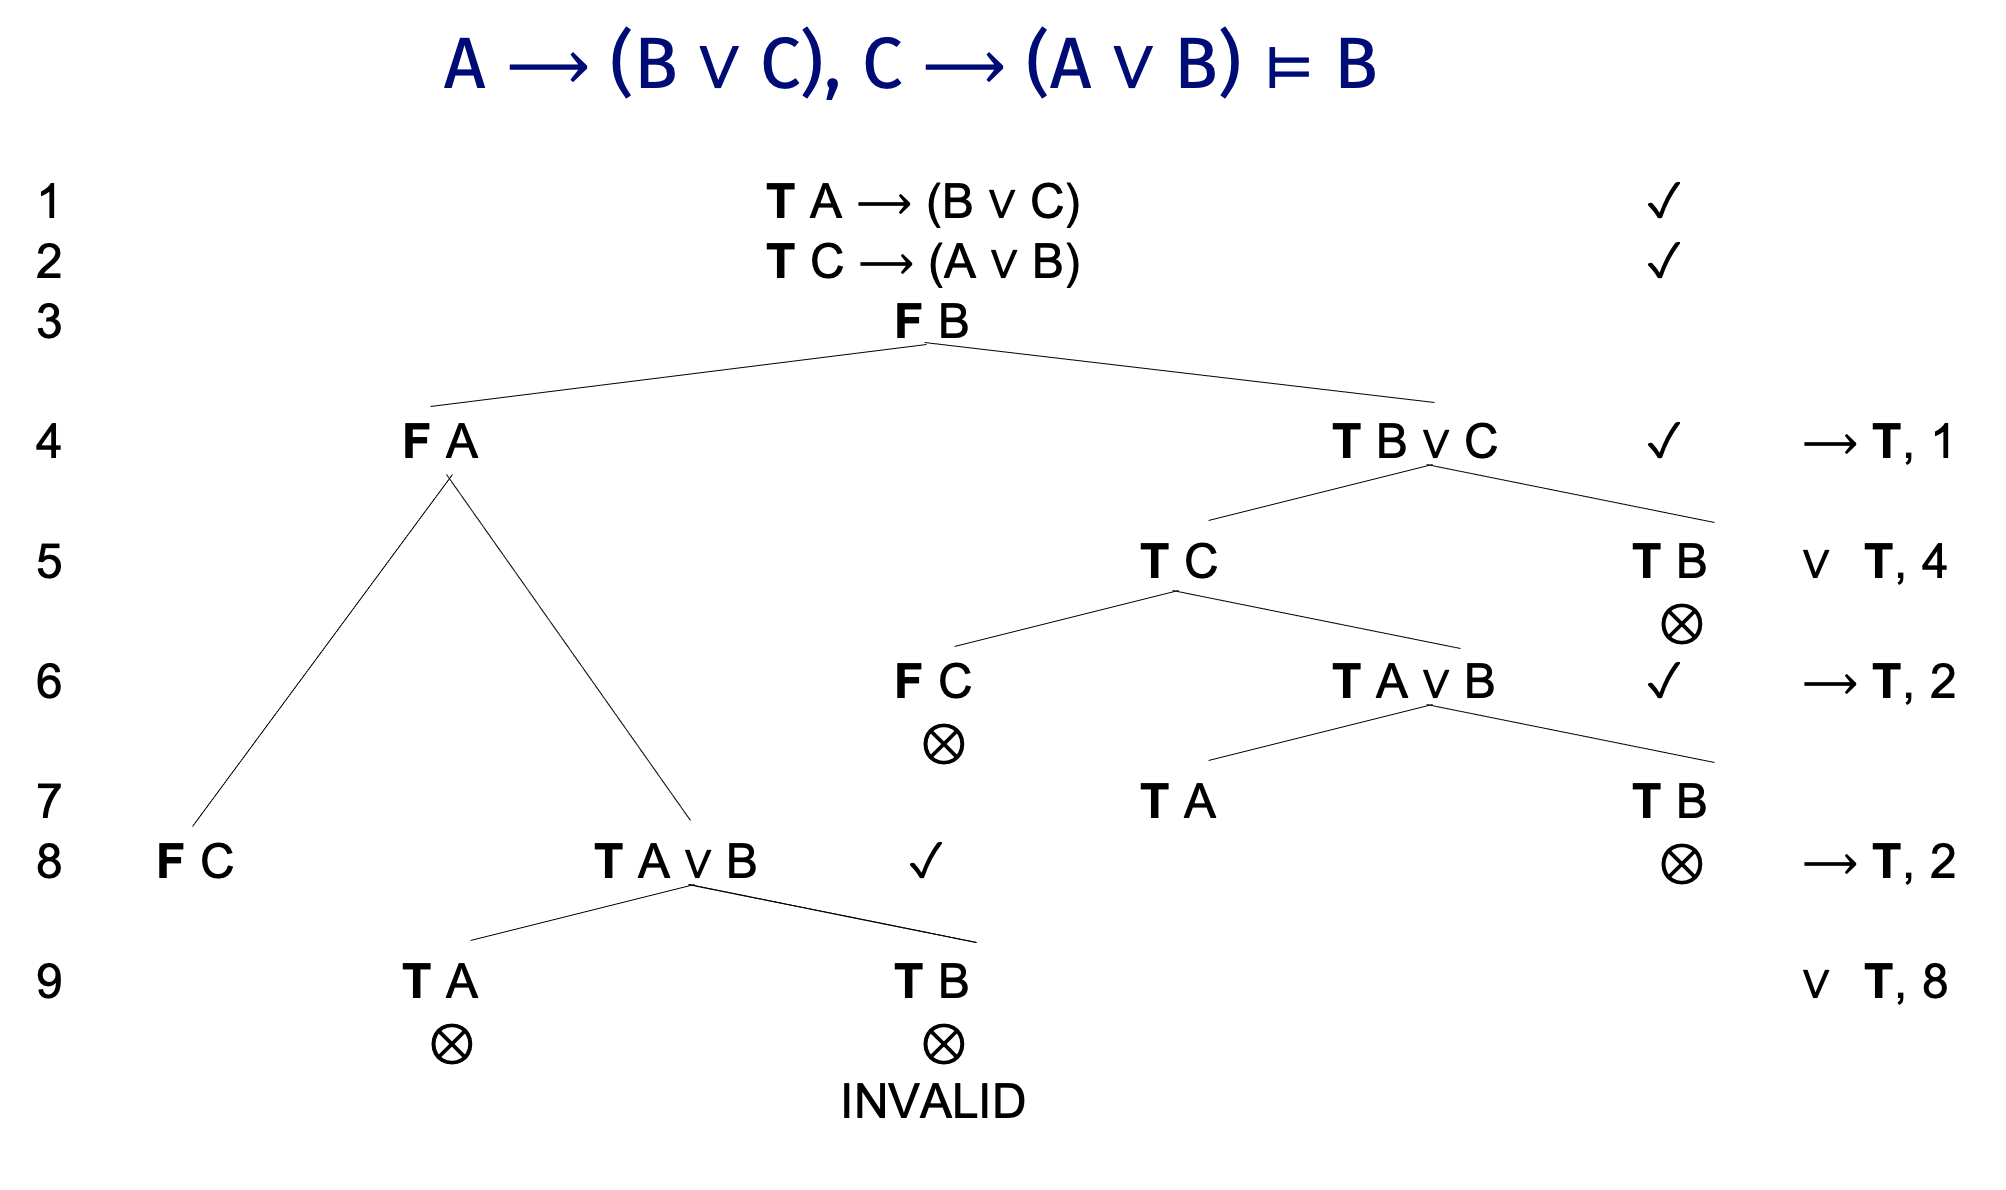
\includegraphics{q08.png}

\newpage

\hypertarget{proofs}{%
\subsection{Proofs}\label{proofs}}

Construct a proof for each of the following

\begin{enumerate}
\def\labelenumi{\arabic{enumi}.}
\setcounter{enumi}{8}
\tightlist
\item
  \(P \rightarrow (Q \wedge R), S \wedge P \vdash R \wedge (S \vee T)\)
\end{enumerate}

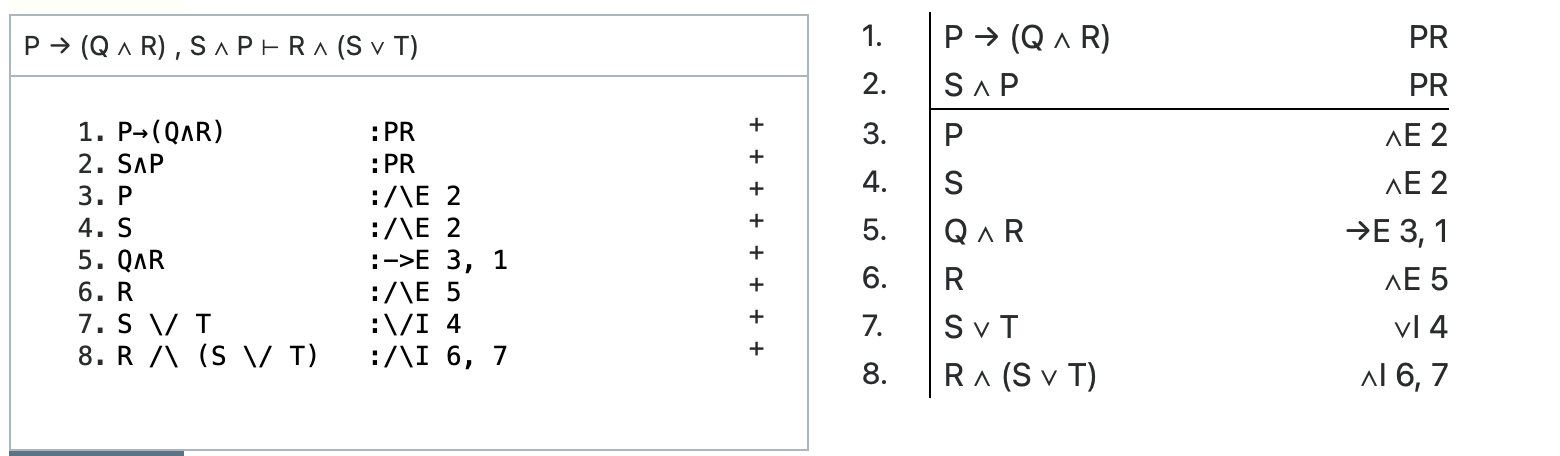
\includegraphics{q09.png}

\begin{enumerate}
\def\labelenumi{\arabic{enumi}.}
\setcounter{enumi}{9}
\tightlist
\item
  \((P \wedge Q) \rightarrow R \vdash P \rightarrow (Q \rightarrow R)\)
\end{enumerate}

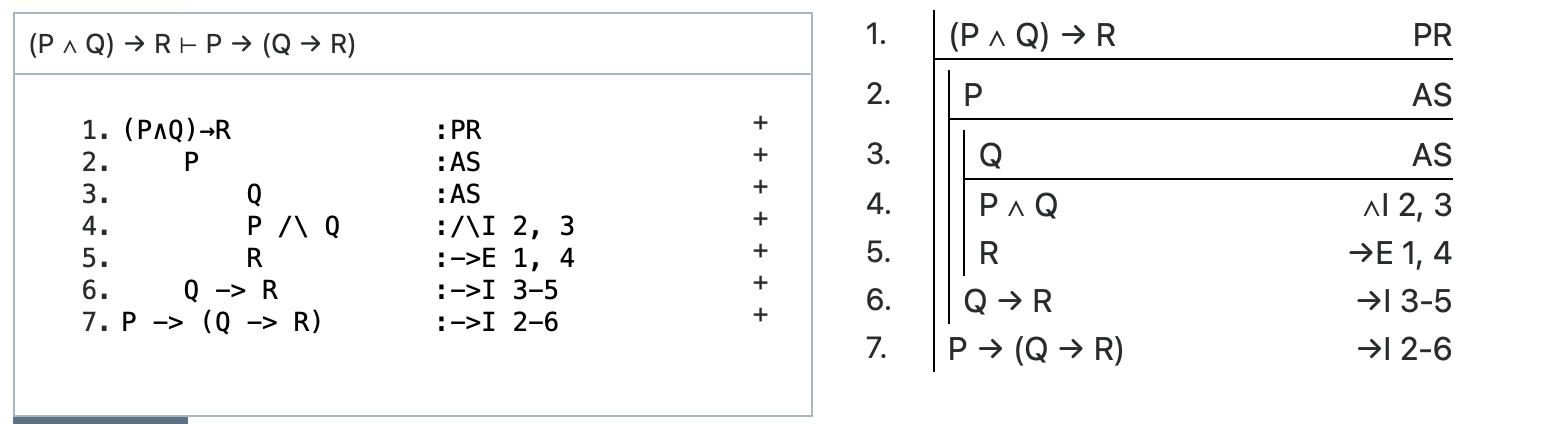
\includegraphics{q10.png}

\begin{enumerate}
\def\labelenumi{\arabic{enumi}.}
\setcounter{enumi}{10}
\tightlist
\item
  \(P \rightarrow R, Q \rightarrow R \vdash (P \vee Q) \rightarrow R\)
\end{enumerate}

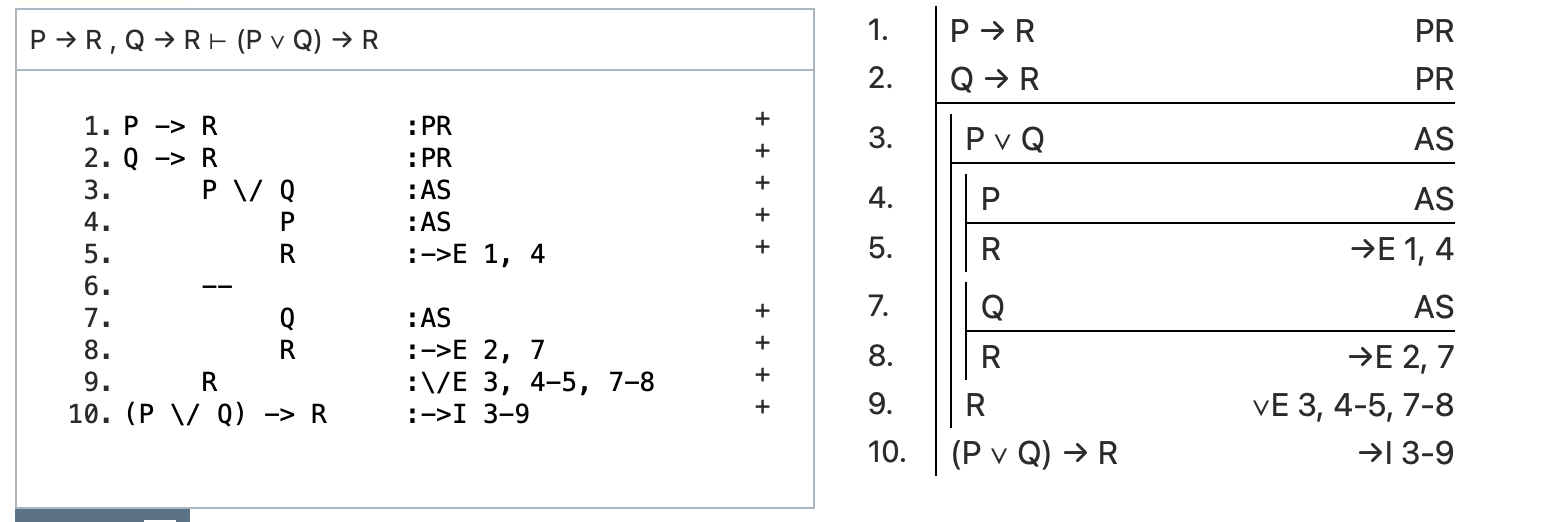
\includegraphics{q11.png}

\newpage

\begin{enumerate}
\def\labelenumi{\arabic{enumi}.}
\setcounter{enumi}{11}
\tightlist
\item
  \(P \rightarrow (Q \wedge R), P \rightarrow (R \rightarrow \neg Q) \vdash \neg P\)
\end{enumerate}

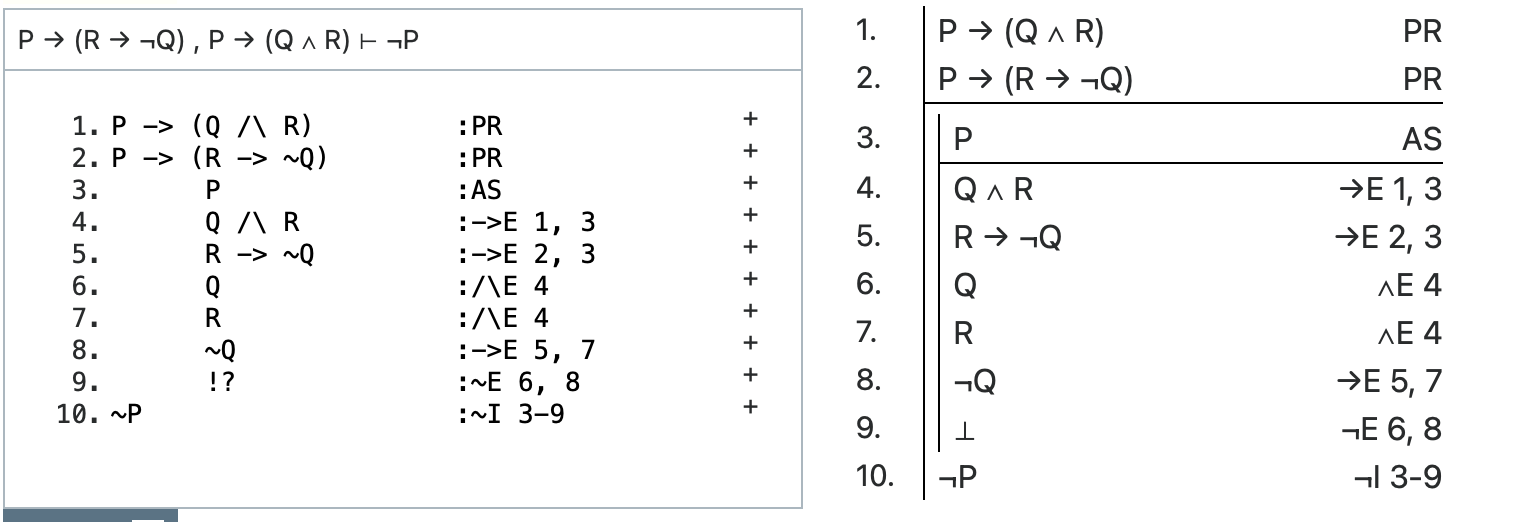
\includegraphics{q12.png}

\hypertarget{probability}{%
\subsection{Probability}\label{probability}}

\begin{enumerate}
\def\labelenumi{\arabic{enumi}.}
\setcounter{enumi}{12}
\tightlist
\item
  A fair coin (with equal chance of landing heads and landing tails) is
  about to be flipped. Ankita is offered the following bet - if it lands
  heads she wins \$200, and if it lands tails she loses \$100. Do we
  know enough to advise Ankita whether or not she should take the bet?
  Why or why not?
\end{enumerate}

\emph{We do not know enough. We need to know the utility of gaining
\$200 and of losing \$100, and which of these is larger. The theory
doesn't tell us these; it's up to her how much she values these things.
So as it stands, we don't know enough to advise her}.

\begin{enumerate}
\def\labelenumi{\arabic{enumi}.}
\setcounter{enumi}{13}
\tightlist
\item
  Explain why the following decision rule is not generally reasonable:
  Identity the most likely state; then choose an act which maximizes
  utility in that state. (Hint: Describe a situation where this would
  lead to doing something unreasonable.)
\end{enumerate}

\emph{Consider a choice with the following table, where state A has
probability 0.6, and state B has probability 0.4.}

\begin{longtable}[]{@{}lcc@{}}
\toprule
Options & State A & State B \\
\midrule
\endhead
Option X & 1 & -100000 \\
Option Y & 0 & 0 \\
\bottomrule
\end{longtable}

\emph{The most likely outcome is A. And in A, X is the best option. But
doing X is not in fact reasonable. Here is a real life case of this.
You're driving, and the light ahead is red. There are cars on the cross
street. But they aren't travelling fast, and if you just run the red
light they'll probably stop. Probably. But running the light has a
marginal gain, and if you're wrong about whether they'll stop, it would
be catastrophic. You should stop, even though in the most likely state
of the world (where the other cars avoid you), you would be (very
slightly!) better off running the light.}

\hypertarget{modal-logic}{%
\subsection{Modal Logic}\label{modal-logic}}

For each of the following sentences, do \textbf{three} truth trees: one
to check whether it is a logical truth in K, one to check whether it is
a logical truth in S4, and one to check whether it is a logical truth in
KT4B (i.e., S5). You can use the simplified rules for S5.

\begin{enumerate}
\def\labelenumi{\arabic{enumi}.}
\setcounter{enumi}{14}
\tightlist
\item
  \(\Box(\Box A \rightarrow B) \vee \Box A\)
\end{enumerate}

It is invalid in K.

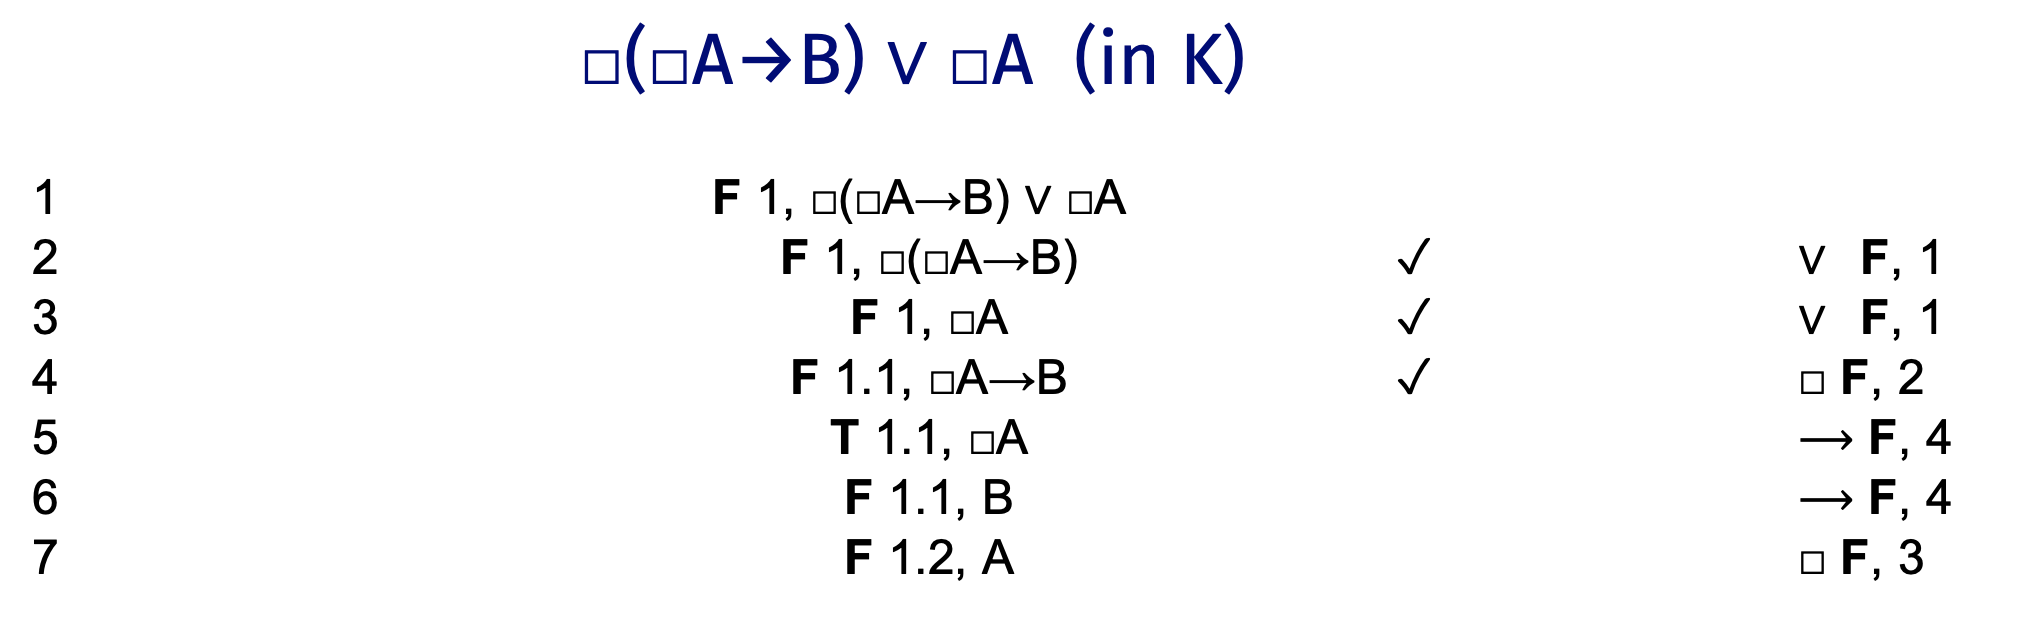
\includegraphics{q15a.png}

It is invalid in S4.

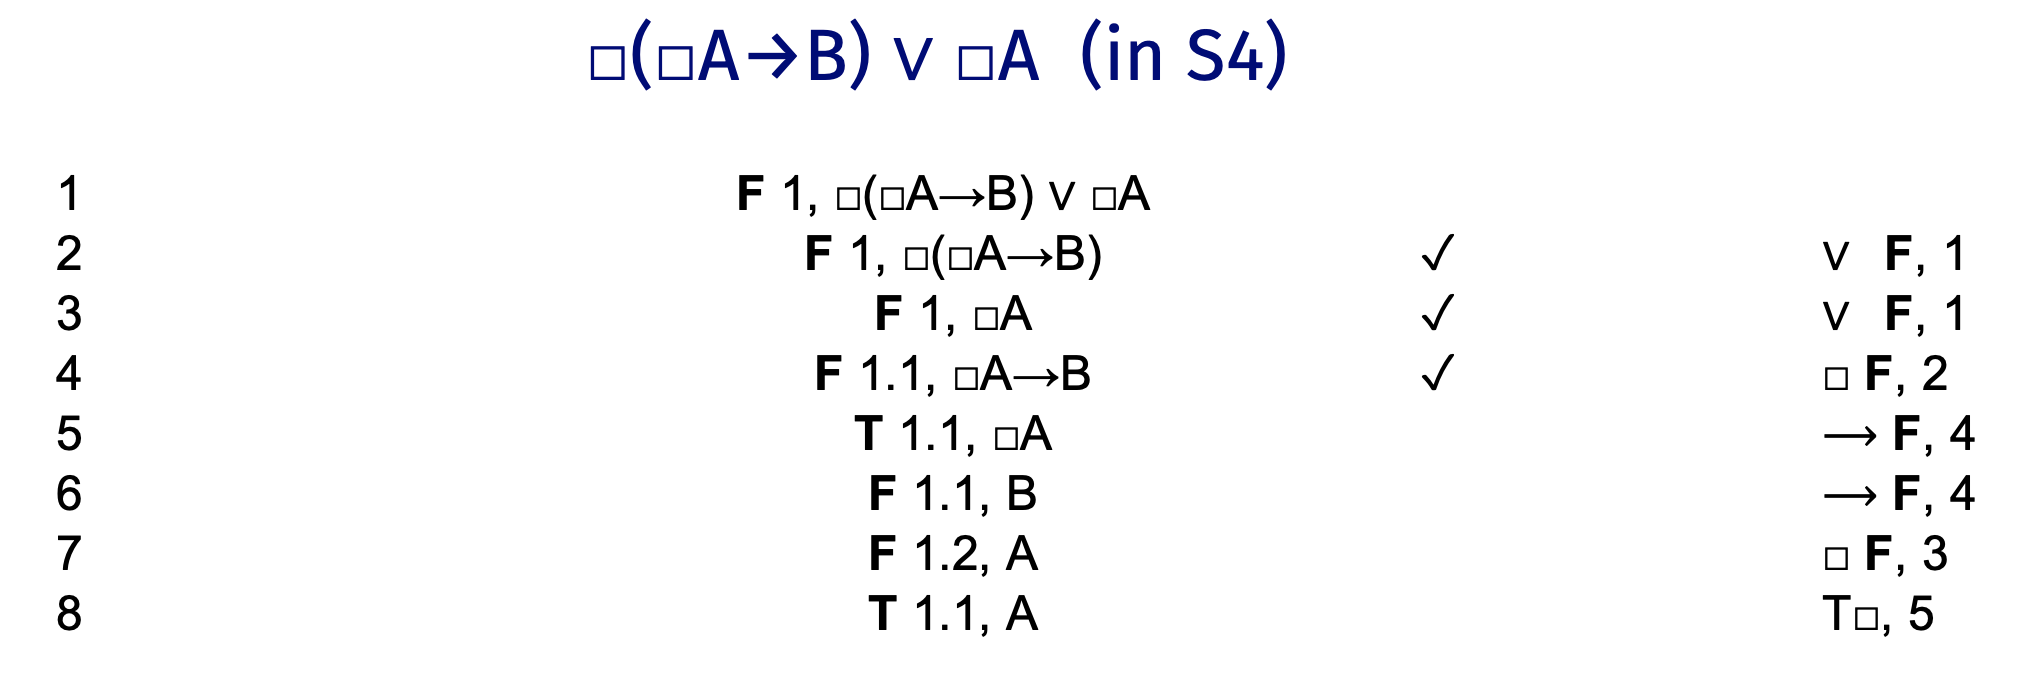
\includegraphics{q15b.png}

It is valid in S5.

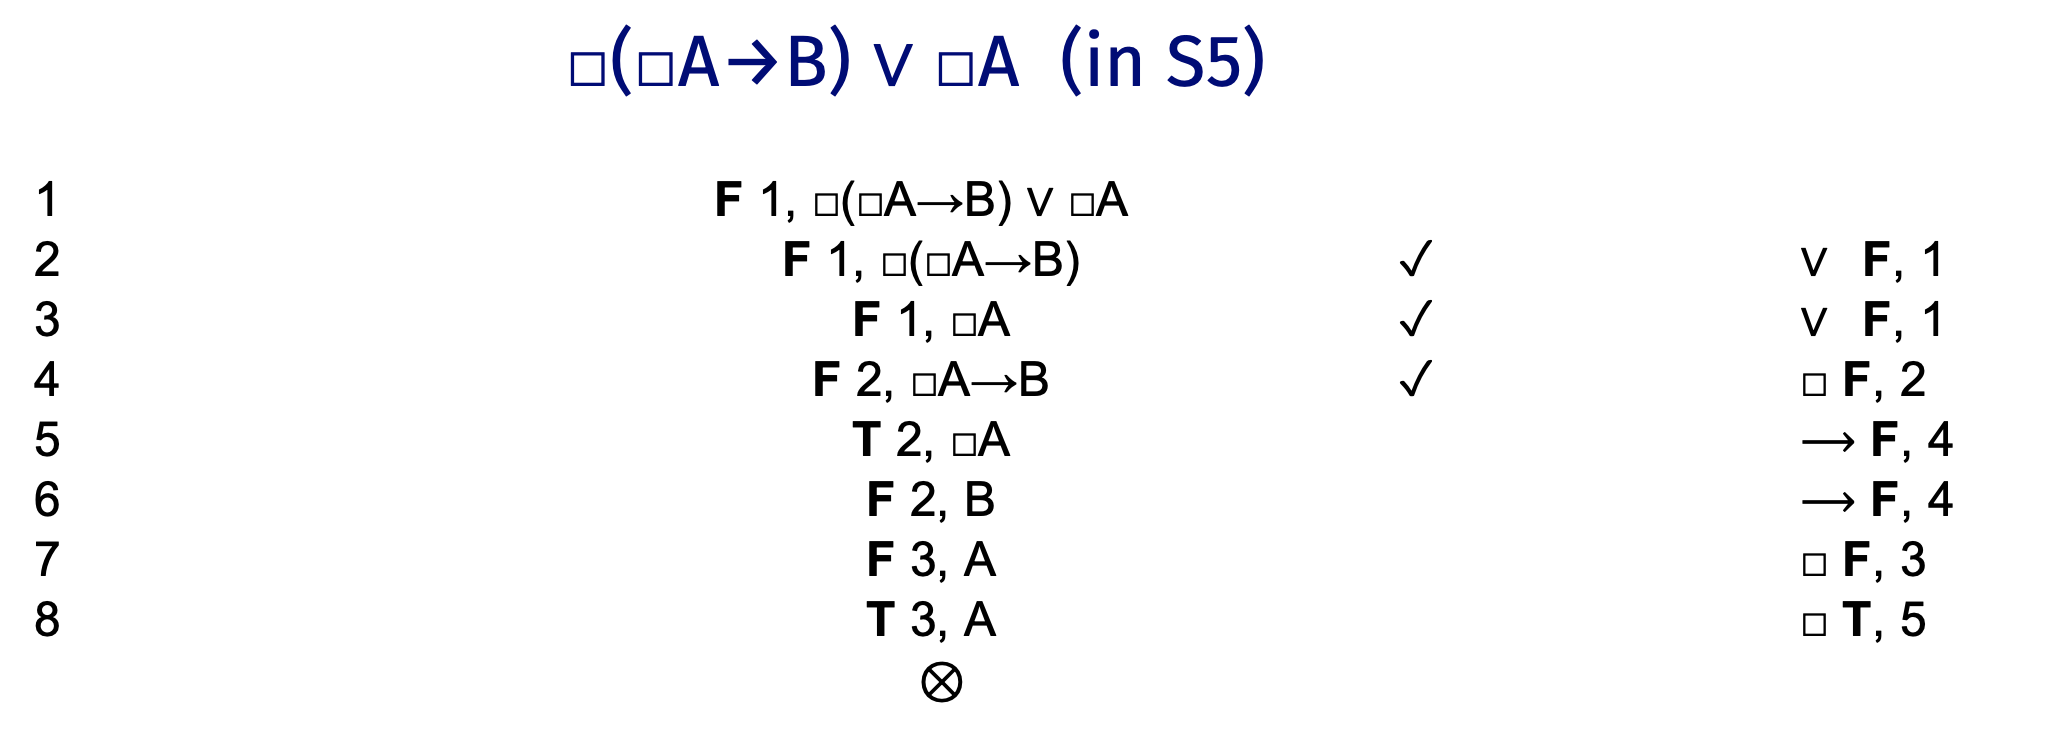
\includegraphics{q15c.png}

\begin{enumerate}
\def\labelenumi{\arabic{enumi}.}
\setcounter{enumi}{15}
\tightlist
\item
  \(\Diamond(A \rightarrow \Diamond \Box A)\)
\end{enumerate}

It is invalid in K.


\includegraphics{q16a.png}

It is valid in S4, and this tree also shows it is valid in S5.

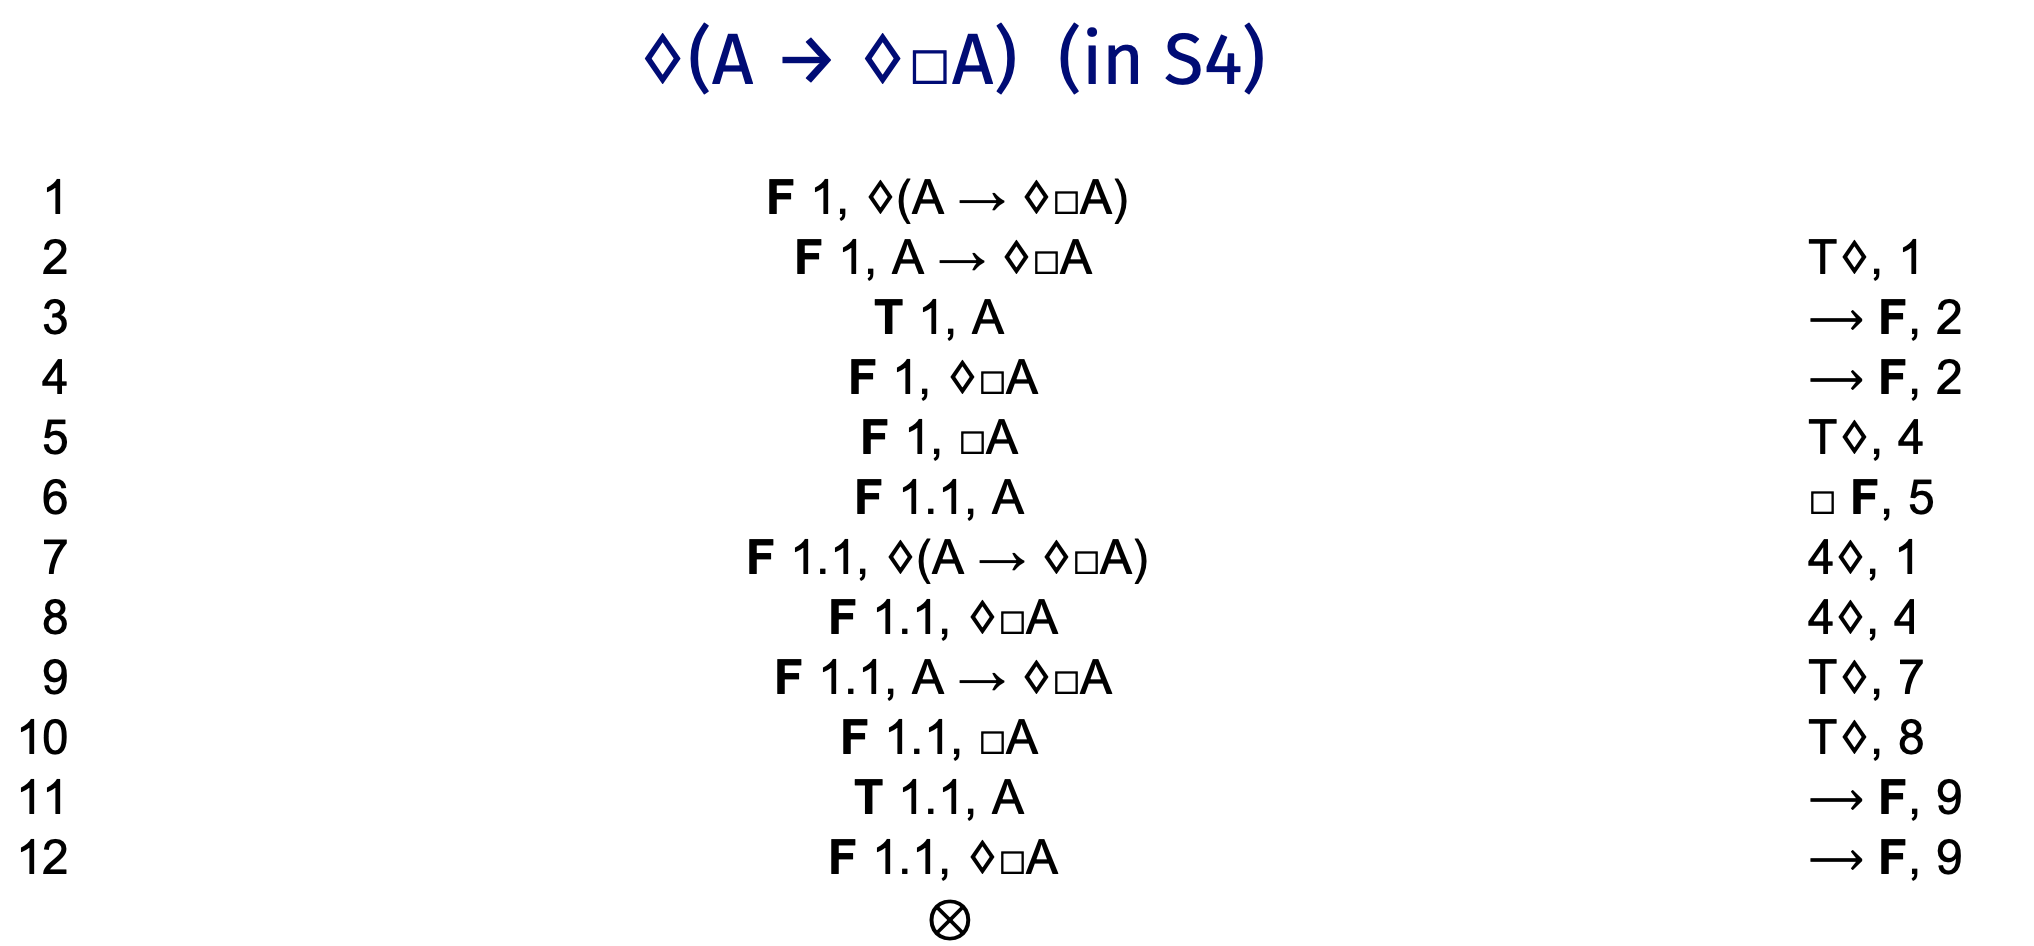
\includegraphics{q16b.png}

\hypertarget{conditionals}{%
\subsection{Conditionals}\label{conditionals}}

\begin{enumerate}
\def\labelenumi{\arabic{enumi}.}
\setcounter{enumi}{16}
\tightlist
\item
  Show that
  \(\Box (A \rightarrow B) \rightarrow \Box ((A \wedge C) \rightarrow B)\)
  is a theorem of S5.
\end{enumerate}

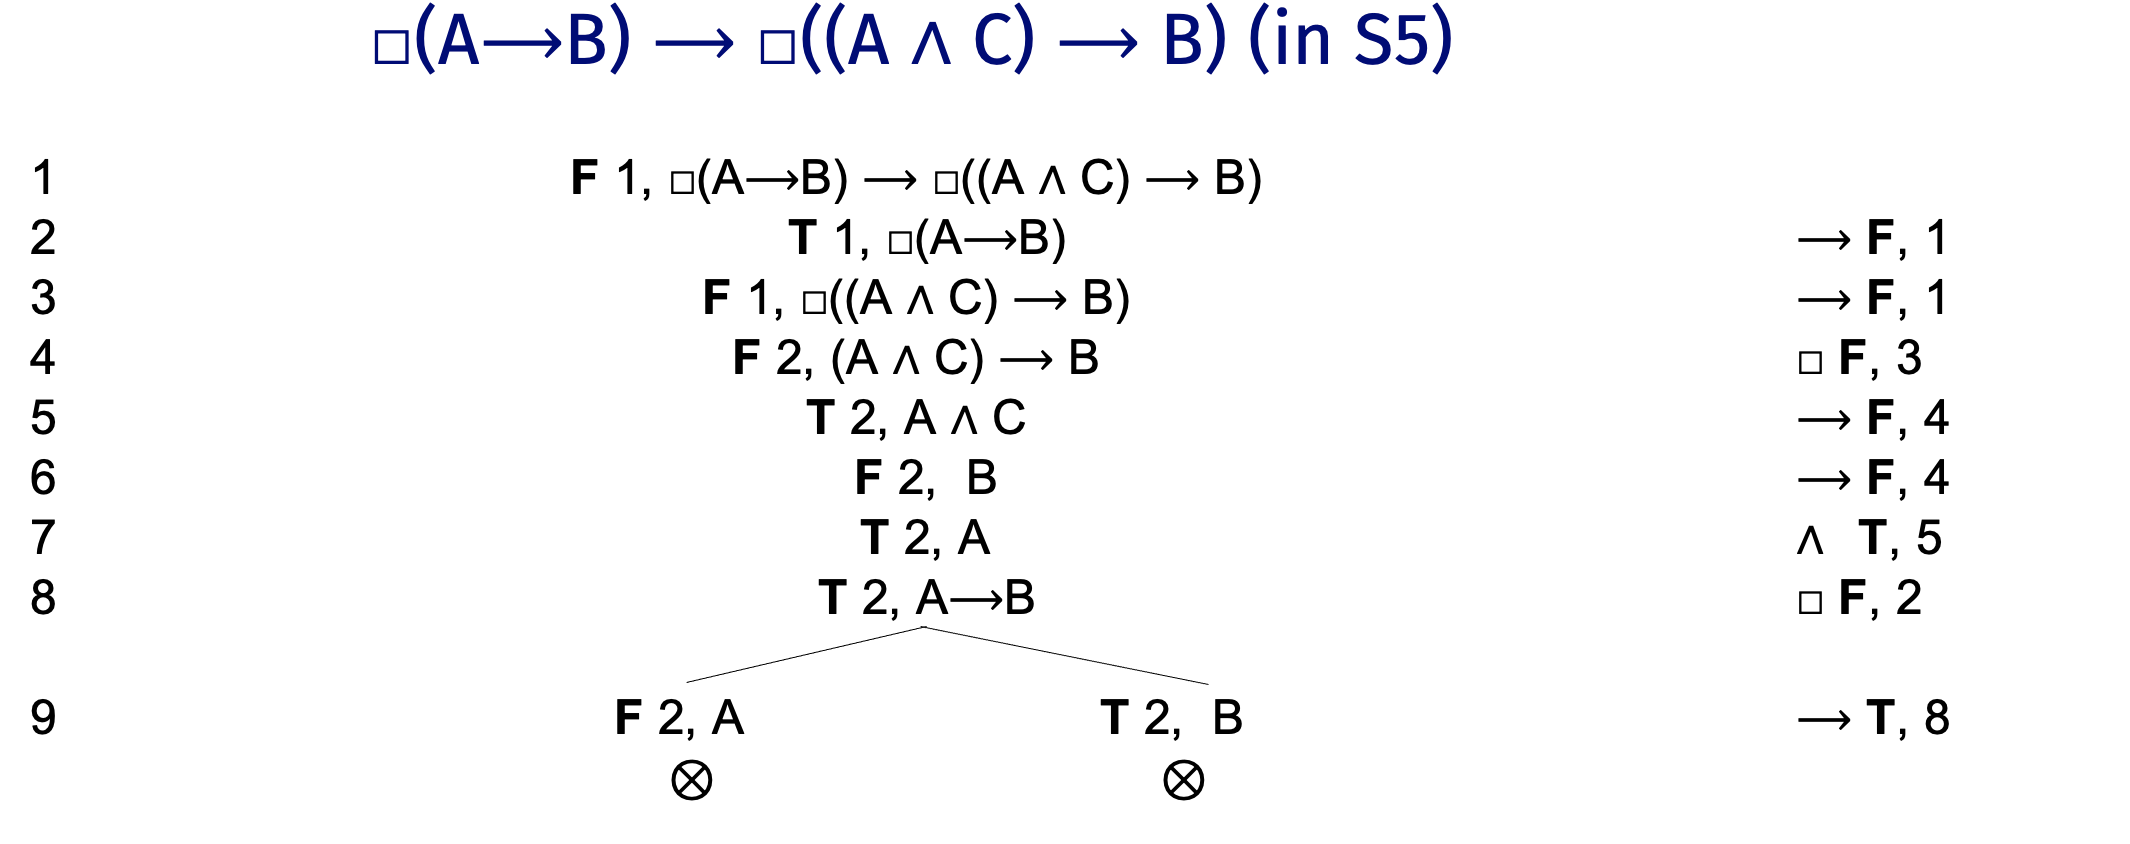
\includegraphics{q17.png}

\newpage

\begin{enumerate}
\def\labelenumi{\arabic{enumi}.}
\setcounter{enumi}{17}
\tightlist
\item
  Describe a sphere model (from the minimal change semantics chapter of
  \emph{Boxes And Diamonds}) that shows
  \(((A \boxright B) \wedge (B \boxright C)) \rightarrow (A \boxright C)\)
  is not a logical truth in the minimal change semantics.
\end{enumerate}

\emph{In words, here is a model. In the actual world, A, B, C are all
false. The nearest world where A is true is 10 units away, and at it B
is true and C is false. The nearest world where B is true is 5 units
away, and at it A is false and C is true.}

\emph{Here is a picture that shows the same model. (You only need to do
either a picture or a model. And any drawing that's clear will be fine -
you don't need anything like these graphics.)}

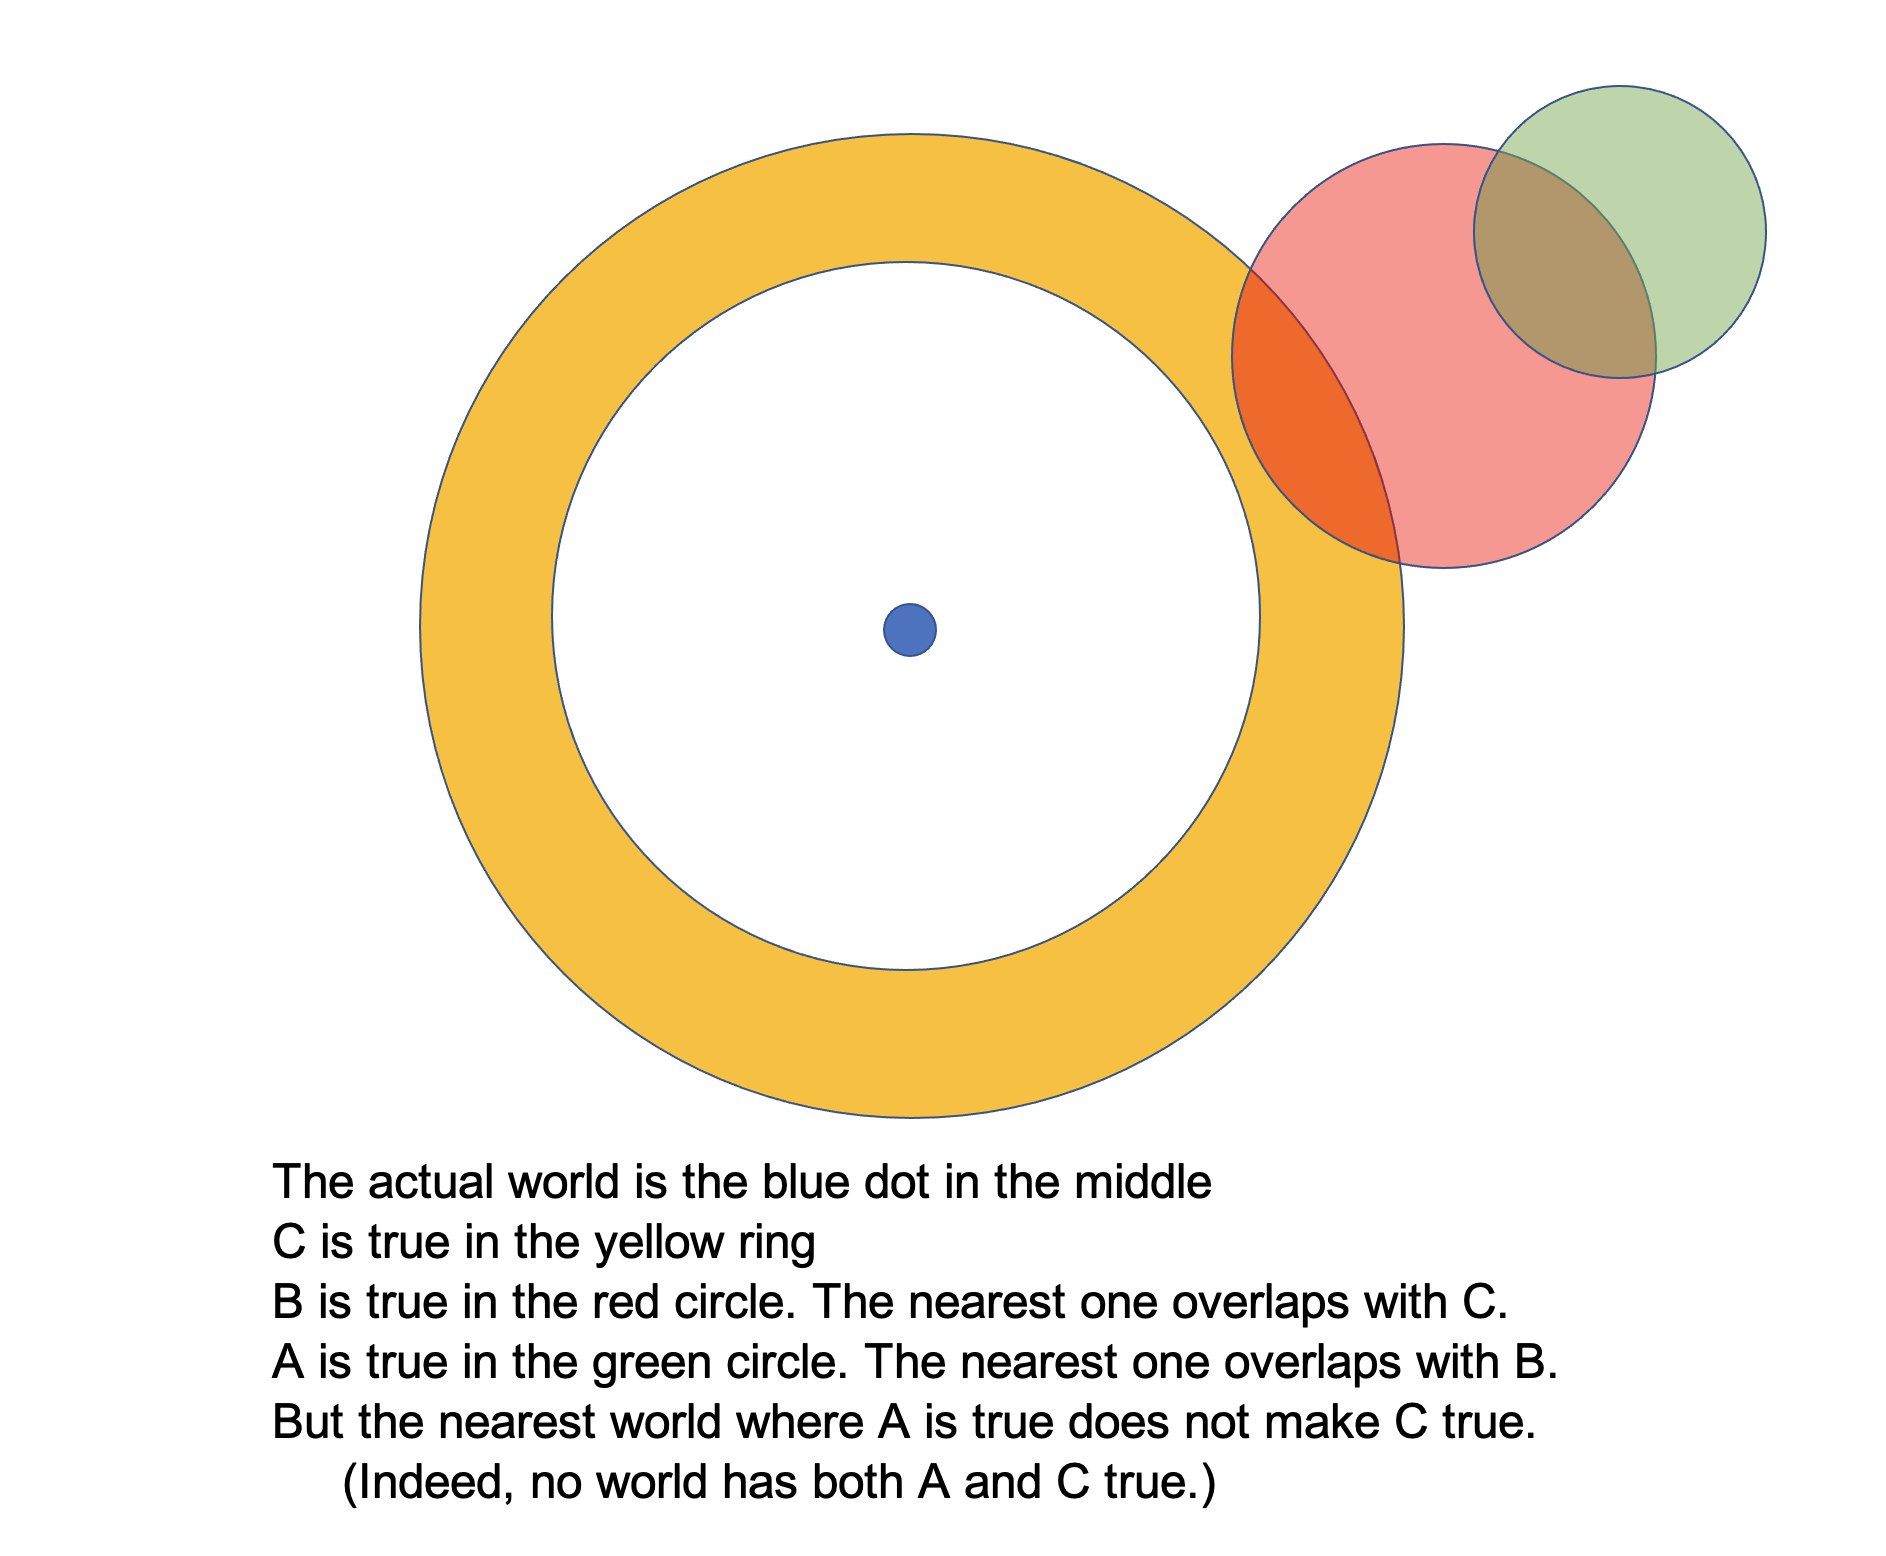
\includegraphics{q18.png}

\end{document}
